\documentclass[]{article}
\usepackage{lmodern}
\usepackage{amssymb,amsmath}
\usepackage{ifxetex,ifluatex}
\usepackage{fixltx2e} % provides \textsubscript
\ifnum 0\ifxetex 1\fi\ifluatex 1\fi=0 % if pdftex
  \usepackage[T1]{fontenc}
  \usepackage[utf8]{inputenc}
\else % if luatex or xelatex
  \ifxetex
    \usepackage{mathspec}
  \else
    \usepackage{fontspec}
  \fi
  \defaultfontfeatures{Ligatures=TeX,Scale=MatchLowercase}
\fi
% use upquote if available, for straight quotes in verbatim environments
\IfFileExists{upquote.sty}{\usepackage{upquote}}{}
% use microtype if available
\IfFileExists{microtype.sty}{%
\usepackage{microtype}
\UseMicrotypeSet[protrusion]{basicmath} % disable protrusion for tt fonts
}{}
\usepackage[left=1.1in, right=1.1in, top=1.1in, bottom=1.1in]{geometry}
\usepackage{hyperref}
\hypersetup{unicode=true,
            pdftitle={Stat 435 Lecture Notes 6},
            pdfauthor={Xiongzhi Chen; Washington State University},
            pdfborder={0 0 0},
            breaklinks=true}
\urlstyle{same}  % don't use monospace font for urls
\usepackage{color}
\usepackage{fancyvrb}
\newcommand{\VerbBar}{|}
\newcommand{\VERB}{\Verb[commandchars=\\\{\}]}
\DefineVerbatimEnvironment{Highlighting}{Verbatim}{commandchars=\\\{\}}
% Add ',fontsize=\small' for more characters per line
\usepackage{framed}
\definecolor{shadecolor}{RGB}{248,248,248}
\newenvironment{Shaded}{\begin{snugshade}}{\end{snugshade}}
\newcommand{\KeywordTok}[1]{\textcolor[rgb]{0.13,0.29,0.53}{\textbf{{#1}}}}
\newcommand{\DataTypeTok}[1]{\textcolor[rgb]{0.13,0.29,0.53}{{#1}}}
\newcommand{\DecValTok}[1]{\textcolor[rgb]{0.00,0.00,0.81}{{#1}}}
\newcommand{\BaseNTok}[1]{\textcolor[rgb]{0.00,0.00,0.81}{{#1}}}
\newcommand{\FloatTok}[1]{\textcolor[rgb]{0.00,0.00,0.81}{{#1}}}
\newcommand{\ConstantTok}[1]{\textcolor[rgb]{0.00,0.00,0.00}{{#1}}}
\newcommand{\CharTok}[1]{\textcolor[rgb]{0.31,0.60,0.02}{{#1}}}
\newcommand{\SpecialCharTok}[1]{\textcolor[rgb]{0.00,0.00,0.00}{{#1}}}
\newcommand{\StringTok}[1]{\textcolor[rgb]{0.31,0.60,0.02}{{#1}}}
\newcommand{\VerbatimStringTok}[1]{\textcolor[rgb]{0.31,0.60,0.02}{{#1}}}
\newcommand{\SpecialStringTok}[1]{\textcolor[rgb]{0.31,0.60,0.02}{{#1}}}
\newcommand{\ImportTok}[1]{{#1}}
\newcommand{\CommentTok}[1]{\textcolor[rgb]{0.56,0.35,0.01}{\textit{{#1}}}}
\newcommand{\DocumentationTok}[1]{\textcolor[rgb]{0.56,0.35,0.01}{\textbf{\textit{{#1}}}}}
\newcommand{\AnnotationTok}[1]{\textcolor[rgb]{0.56,0.35,0.01}{\textbf{\textit{{#1}}}}}
\newcommand{\CommentVarTok}[1]{\textcolor[rgb]{0.56,0.35,0.01}{\textbf{\textit{{#1}}}}}
\newcommand{\OtherTok}[1]{\textcolor[rgb]{0.56,0.35,0.01}{{#1}}}
\newcommand{\FunctionTok}[1]{\textcolor[rgb]{0.00,0.00,0.00}{{#1}}}
\newcommand{\VariableTok}[1]{\textcolor[rgb]{0.00,0.00,0.00}{{#1}}}
\newcommand{\ControlFlowTok}[1]{\textcolor[rgb]{0.13,0.29,0.53}{\textbf{{#1}}}}
\newcommand{\OperatorTok}[1]{\textcolor[rgb]{0.81,0.36,0.00}{\textbf{{#1}}}}
\newcommand{\BuiltInTok}[1]{{#1}}
\newcommand{\ExtensionTok}[1]{{#1}}
\newcommand{\PreprocessorTok}[1]{\textcolor[rgb]{0.56,0.35,0.01}{\textit{{#1}}}}
\newcommand{\AttributeTok}[1]{\textcolor[rgb]{0.77,0.63,0.00}{{#1}}}
\newcommand{\RegionMarkerTok}[1]{{#1}}
\newcommand{\InformationTok}[1]{\textcolor[rgb]{0.56,0.35,0.01}{\textbf{\textit{{#1}}}}}
\newcommand{\WarningTok}[1]{\textcolor[rgb]{0.56,0.35,0.01}{\textbf{\textit{{#1}}}}}
\newcommand{\AlertTok}[1]{\textcolor[rgb]{0.94,0.16,0.16}{{#1}}}
\newcommand{\ErrorTok}[1]{\textcolor[rgb]{0.64,0.00,0.00}{\textbf{{#1}}}}
\newcommand{\NormalTok}[1]{{#1}}
\usepackage{graphicx,grffile}
\makeatletter
\def\maxwidth{\ifdim\Gin@nat@width>\linewidth\linewidth\else\Gin@nat@width\fi}
\def\maxheight{\ifdim\Gin@nat@height>\textheight\textheight\else\Gin@nat@height\fi}
\makeatother
% Scale images if necessary, so that they will not overflow the page
% margins by default, and it is still possible to overwrite the defaults
% using explicit options in \includegraphics[width, height, ...]{}
\setkeys{Gin}{width=\maxwidth,height=\maxheight,keepaspectratio}
\IfFileExists{parskip.sty}{%
\usepackage{parskip}
}{% else
\setlength{\parindent}{0pt}
\setlength{\parskip}{6pt plus 2pt minus 1pt}
}
\setlength{\emergencystretch}{3em}  % prevent overfull lines
\providecommand{\tightlist}{%
  \setlength{\itemsep}{0pt}\setlength{\parskip}{0pt}}
\setcounter{secnumdepth}{0}
% Redefines (sub)paragraphs to behave more like sections
\ifx\paragraph\undefined\else
\let\oldparagraph\paragraph
\renewcommand{\paragraph}[1]{\oldparagraph{#1}\mbox{}}
\fi
\ifx\subparagraph\undefined\else
\let\oldsubparagraph\subparagraph
\renewcommand{\subparagraph}[1]{\oldsubparagraph{#1}\mbox{}}
\fi

%%% Use protect on footnotes to avoid problems with footnotes in titles
\let\rmarkdownfootnote\footnote%
\def\footnote{\protect\rmarkdownfootnote}

%%% Change title format to be more compact
\usepackage{titling}

% Create subtitle command for use in maketitle
\newcommand{\subtitle}[1]{
  \posttitle{
    \begin{center}\large#1\end{center}
    }
}

\setlength{\droptitle}{-2em}

  \title{Stat 435 Lecture Notes 6}
    \pretitle{\vspace{\droptitle}\centering\huge}
  \posttitle{\par}
    \author{Xiongzhi Chen \\ Washington State University}
    \preauthor{\centering\large\emph}
  \postauthor{\par}
    \date{}
    \predate{}\postdate{}
  
\usepackage{bbm}
\usepackage{amssymb}
\usepackage{amsmath}
\usepackage{graphicx,float}

\begin{document}
\maketitle

{
\setcounter{tocdepth}{2}
\tableofcontents
}
\section{}\label{section}

\subsection{Topics to discuss}\label{topics-to-discuss}

\begin{itemize}
\tightlist
\item
  Multinomial regression
\item
  Poisson regression
\end{itemize}

\section{Multinomial regression}\label{multinomial-regression}

\subsection{Observations in classes}\label{observations-in-classes}

Each observations \(y_i,i=1,\cdots,n\) belongs to one and only one of
\(K\) classes:

\begin{itemize}
\tightlist
\item
  Class \(1\) obs: \(\tilde{y}_{11}\),\(\tilde{y}_{12}\),\(\cdots\),
  \(\tilde{y}_{1,n_{1}}\)
\item
  Class \(2\) obs: \(\tilde{y}_{21}\),\(\tilde{y}_{22}\),\(\cdots\),
  \(\tilde{y}_{2,n_{2}}\)
\item
  Class \ldots{} obs
\item
  Class \(K\) obs: \(\tilde{y}_{K1}\),\(\tilde{y}_{K2}\),\(\cdots\),
  \(\tilde{y}_{K,n_{K}}\)
\end{itemize}

\subsection{Probability mass function}\label{probability-mass-function}

\begin{itemize}
\tightlist
\item
  Model: \(P(y_i=k) = p_{ik}\)
\item
  Equivalent formulation: set \(y_{ij}=1\) if and only if \(y_{i}=j\).
  Then \emph{probability mass function (pmf)}
\end{itemize}

\[P(y_i=k) = p_{i1}^{y_{i1}}\cdots p_{ik}^{y_{ik}}\cdots
p_{iK}^{y_{iK}}=\prod_{j=1}^{K}p_{ij}^{y_{ij}}\]

\begin{itemize}
\item
  Example with \(K=3\); comparison with Bernoulli setting
\item
  When \(\left\{ y_{i}\right\} _{i=1}^{n}\) are independent, their joint
  likelihood is \[
  L=\prod_{i=1}^{n}p_{i1}^{y_{i1}}\cdots p_{ik}^{y_{ik}}\cdots p_{iK}^{y_{iK}%
  }=\prod_{i=1}^{n}\prod_{j=1}^{K}p_{ij}^{y_{ij}}%
  \]
\end{itemize}

\subsection{Model}\label{model}

\begin{itemize}
\tightlist
\item
  \(Y \in \left\{ 1,2,...,K\right\}\) such that \[
  \sum_{k=1}^{K}\Pr\left(  Y=k\right)  =1\text{ and }\prod_{k=1}^{K}\Pr\left(
  Y=k\right)  >0
  \]
\item
  Model \(\Pr\left( Y=k\right)\) by
  \(X=\left( X_{1},X_{2},...,X_{p}\right) ^{T}\)

  \begin{itemize}
  \tightlist
  \item
    Set \(p_{k}\left( X\right) =\Pr(Y=k|X)\) for \(k=1,\ldots,K\)
  \item
    For \(k=1,\ldots,K-1\), set

    \begin{equation}
    \log\left(  \frac{p_{k}\left(  X\right)  }{p_{K}\left(  X\right)  }\right)
    =\beta_{k0}+\beta_{k}^{T}X, 
    \end{equation}

    where
    \(\beta_{k}=\left( \beta_{k1},\beta_{k2},...,\beta_{kp}\right) ^{T}\)
  \end{itemize}
\end{itemize}

\subsection{Equivalent model}\label{equivalent-model}

Model is equivalent to:

\[
p_{k}\left(  x\right) = \Pr(Y=k|X=x)=\frac{\beta_{k0}+\beta_{k}^{T}x}{1+\sum_{l=1}^{K-1}\exp(\beta_{l0}+\beta_{l}^{T}x)}
\] for \(k=1,\ldots,K-1\) and \[
p_{K}\left(  x\right) =\Pr(Y=K|X=x)=\frac{1}{1+\sum_{l=1}^{K-1}\exp(\beta_{l0}+\beta_{l}^{T}x)}
\]

\subsection{Model: sample version}\label{model-sample-version}

\begin{itemize}
\tightlist
\item
  The modeling strategy \[
  \log\left(  \frac{p_{k}\left(  x_i\right)  }{p_{K}\left(  x_i\right)  }\right)
  =\beta_{k0}+\beta_{k}^{T}x_{i}
  \] is equivalent to the formulation provided by \texttt{glmnet} as \[
  P\left(  y_{i}=k|X=x_{i}\right)  =\frac{\exp\left(  \tilde{\beta}_{k0}
  +\tilde{\beta}_{k}^{T}x_{i}\right)  }{\sum_{l=1}^{K}\exp\left(  \tilde{\beta
  }_{l0}+\tilde{\beta}_{l}^{T}x_{i}\right)  }%
  \]
\end{itemize}

\subsection{Check on model}\label{check-on-model}

\begin{itemize}
\item
  \texttt{glmnet} fits model: \[
  P\left(  Y=k|X=x\right)  =\frac{\exp\left(  \beta_{k0}+\beta_{k}^{T}x\right)
  }{\sum_{i=1}^{K}\exp\left(  \beta_{k0}+\beta_{k}^{T}x\right)  }\text{ for
  }k=1,...,K
  \]
\item
  To check the linearity assumption, i.e., \[
  \log\frac{P\left(  Y=k|X=x\right)  }{P\left(  Y=K|X=x\right)  }=\exp\left(
  \beta_{k0}+\beta_{k}^{T}x\right)  \text{ for }k=1,...,K-1
  \] we need the estimated coefficients for each class probability
  \(P\left(Y=k|X=x\right)\)
\item
  In general, a goodness-of-fit test for the multinomial logistic
  regression model can be the Pearson's chi-square test or the
  likelihood ratio test
\end{itemize}

\subsection{Check on model}\label{check-on-model-1}

Checking if the multinomial logistic regression assumption is adequate:

\begin{itemize}
\item
  Under suitable conditions,
  \(E\left( y_{i}-\hat{\mu}_{i}\right)\rightarrow0\) as sample size
  \(n\rightarrow\infty\) when no regularization that induces bias in
  \(\hat{\mu}_{i}\) is used in model fitting, where \(\hat{\mu}_{i}\) is
  the estimated mean for \(y_{i}\)
\item
  When LASSO is used, biased is often induced to \(\hat{\mu}_{i}\) as an
  estimate of \(E\left( y_{i}\right)\), and in this case we can only
  have \(E\left(y_{i}-\hat{\mu}_{i}\right)\approx 0\) as
  \(n\rightarrow\infty\)
\end{itemize}

\section{Poisson regression}\label{poisson-regression}

\subsection{Poisson random variable}\label{poisson-random-variable}

\begin{itemize}
\item
  A Poisson random variable \(Y\) is defined via its \emph{pmf} as \[
  \Pr\left(  Y=k\right)  =\frac{\mu^{k}}{k!}e^{-\mu}\text{ for }k\in\left\{
  0,1,2,\ldots\right\}
  \] where \(\mu>0\) is fixed. So,
  \(E\left( Y\right) =V\left( Y\right)=\mu\).
\item
  Given observations \(\left( y_{i},x_{i}\right), i=1,...,n\), set
  \[p\left(  x_{i}\right)  =E\left(  y_{i}|x_{i}\right)  =\mu_{i}\]
\item
  \emph{Poisson linear regression} model: \[
  \log\left(  p\left(  x_{i}\right)  \right)  =\beta_{0}+\beta_{1}x_{i}
  \]
\item
  Above model is equivalent to \[
  \mu_{i}=p\left(  x_{i}\right)  =\exp\left(  \beta_{0}+\beta_{1}x_{i}\right)
  \]
\end{itemize}

\subsection{Model assumptions}\label{model-assumptions}

\begin{itemize}
\item
  Each \(y_{i}\) is a Poisson random variable with mean \(\mu_{i}\)
\item
  \(\log\left( p\left( x_{i}\right) \right)\) is a linear function of
  \(x_{i}\) for \(1\leq i\leq n\)
\item
  The pairs \(\left\{ \left( x_{i},y_{i}\right) \right\}_{i=1}^{n}\) are
  independent
\item
  Joint likelihood function is
  \(L\left(\beta\right) =\prod\nolimits_{i=1}^{n}\frac{\mu_{i}^{y_{i}}}{y_{i}!}e^{-\mu_{i}}\)
  and \[
  \log L\left(  \beta\right)  =\sum_{i=1}^{n}\left[  -\exp\left(  \beta
  _{0}+\beta_{1}x_{i}\right)  \right]  + \\
  \sum_{i=1}^{n}\left[  y_{i}\left(
  \beta_{0}+\beta_{1}x_{i}\right)  -\log\left(  y_{i}!\right)  \right]
  \] with coefficients \(\beta=\left( \beta_{0},\beta_{1}\right)\)
\end{itemize}

\subsection{Estimated model}\label{estimated-model}

\begin{itemize}
\item
  \emph{Maximum likelihood estimate (MLE)}
  \(\hat{\beta}=\left( \hat{\beta}_{0} ,\hat{\beta}_{1}\right)\) of
  \(\beta=\left(\beta_{0},\beta_{1}\right)\) satisfies
  \(\hat{\beta}\in\operatorname*{argmin}_{\beta}L\left( \beta\right)\)
\item
  Predictions on \(y_{i}\) can be made as \[
  \Pr\left(  y_{i}=k|x_{i}\right)  =\frac{\hat{\mu}_{i}^{k}}{k!}e^{-\hat{\mu
  }_{i}}\text{  with }\hat{\mu}_{i}=\exp\left(  \hat{\beta}_{0}+\hat{\beta}
  _{1}x_{i}\right)
  \]
\item
  Namely, \(y_{i}\) is predicted by \(\hat{y}_{i}\) for which \[
  \Pr\left(  \hat{y}_{i}=k|x_{i}\right)  =\frac{\hat{\mu}_{i}^{k}}{k!}e^{-\hat{\mu}_{i}}
  \]
\end{itemize}

\subsection{Model diagnosis}\label{model-diagnosis}

\begin{itemize}
\item
  \emph{Reduced model}
  \(\mu_{i}=p\left( x_{i}\right) =\exp\left( \beta_{0}+\beta_{1}x_{i}\right)\)
  versus \emph{Full model} \(E\left( y_{i}\right) =\mu_{i}\)
\item
  Model deviance is \[
  D   =-2\times\left[  \ln L\left(  \text{Reduced model}\right)  -\ln L\left(
  \text{Full model}\right)  \right] \\
   =-2\left[  \sum_{i=1}^{n}y_{i}\ln\frac{\hat{\mu}_{i}}{y_{i}}+\sum_{i=1}
  ^{n}\left(  y_{i}-\hat{\mu}_{i}\right)  \right]  =\sum_{i=1}^{n}d_{i}^{2}
  \]
\end{itemize}

\subsection{Model diagnosis}\label{model-diagnosis-1}

\begin{itemize}
\tightlist
\item
  Deviance residual \[
  d_{i}=\operatorname{sgn}\left(  y_{i}-\hat{\mu}_{i}\right)  \sqrt{-2y_{i}
  \ln\frac{\hat{\mu}_{i}}{y_{i}}-\left(  y_{i}-\hat{\mu}_{i}\right)  }
  \]
\item
  Pearson residual \[
  r_{i}=\frac{y_{i}-\hat{\mu}_{i}}{\sqrt{\hat{\mu}_{i}}}
  \] and Pearson chi-square goodness of fit statistic \[
  \xi^{2}=\sum_{i=1}^{n}\frac{\left(  y_{i}-\hat{\mu}_{i}\right)  ^{2}}{\hat
  {\mu}_{i}}=\sum_{i=1}^{n}r_{i}^{2}
  \]
\end{itemize}

\subsection{Model diagnosis}\label{model-diagnosis-2}

\begin{itemize}
\tightlist
\item
  Studentized Pearson residual \[
  \tilde{r}_{i}=\frac{r_{i}}{\sqrt{1-h_{ii}}},
  \] where

  \begin{itemize}
  \item
    \(h_{ii}\) is the \(i\)-th diagonal entry of \[
    H=W^{1/2}X\left(  X^{\prime}WX\right)  ^{-1}X^{\prime}W^{1/2}
    \]
  \item
    \(W\) is the \(n\times n\) diagonal matrix with entries
    \(\hat{\mu}_{i}\)
  \item
    \(X\) is the \(n\times p\) design matrix
  \end{itemize}
\end{itemize}

\subsection{Model diagnosis}\label{model-diagnosis-3}

\begin{itemize}
\item
  Poisson model is correct \(\implies\)
  \(E\left( y_{i}-\hat{\mu}_{i}\right) =0\) asymptotically
\item
  Check linearity assumption: plot \(\ln\hat{\mu}_{i}\) against
  \(x_{i}\)
\item
  Check Poisson model adequacy: plot \(r_{i}\) against \(\hat{\mu}_{i}\)
\item
  Check for influential observations: plot \emph{delta chi-square
  statistic} \[
  \Delta\xi_{\left(  i\right)  }^{2}=\xi^{2}-\xi_{\left(  i\right)  }^{2}
  \] and \emph{delta deviance statistic} \[
  \Delta D_{\left(  i\right)  }=D-D_{\left(  i\right)  }
  \] against \(i\) (or against \(\hat{\mu}_{i}\) or \(\hat{\eta}_{i}\))
\end{itemize}

\subsection{Example: data}\label{example-data}

Miller Lumber Company survey data:

\begin{itemize}
\tightlist
\item
  \(X_1\): number of housing units
\item
  \(X_2\): average income, in dollars
\item
  \(X_3\): average housing unit age, in years
\item
  \(X_4\): distance to nearest competitor, in miles
\item
  \(X_5\): distance to store, in miles
\item
  \(Y\): number of customers who visited store from census tract
\end{itemize}

(Credit: authors of book ``Applied linear statistical models'')

\subsection{Example: partial data}\label{example-partial-data}

\begin{center}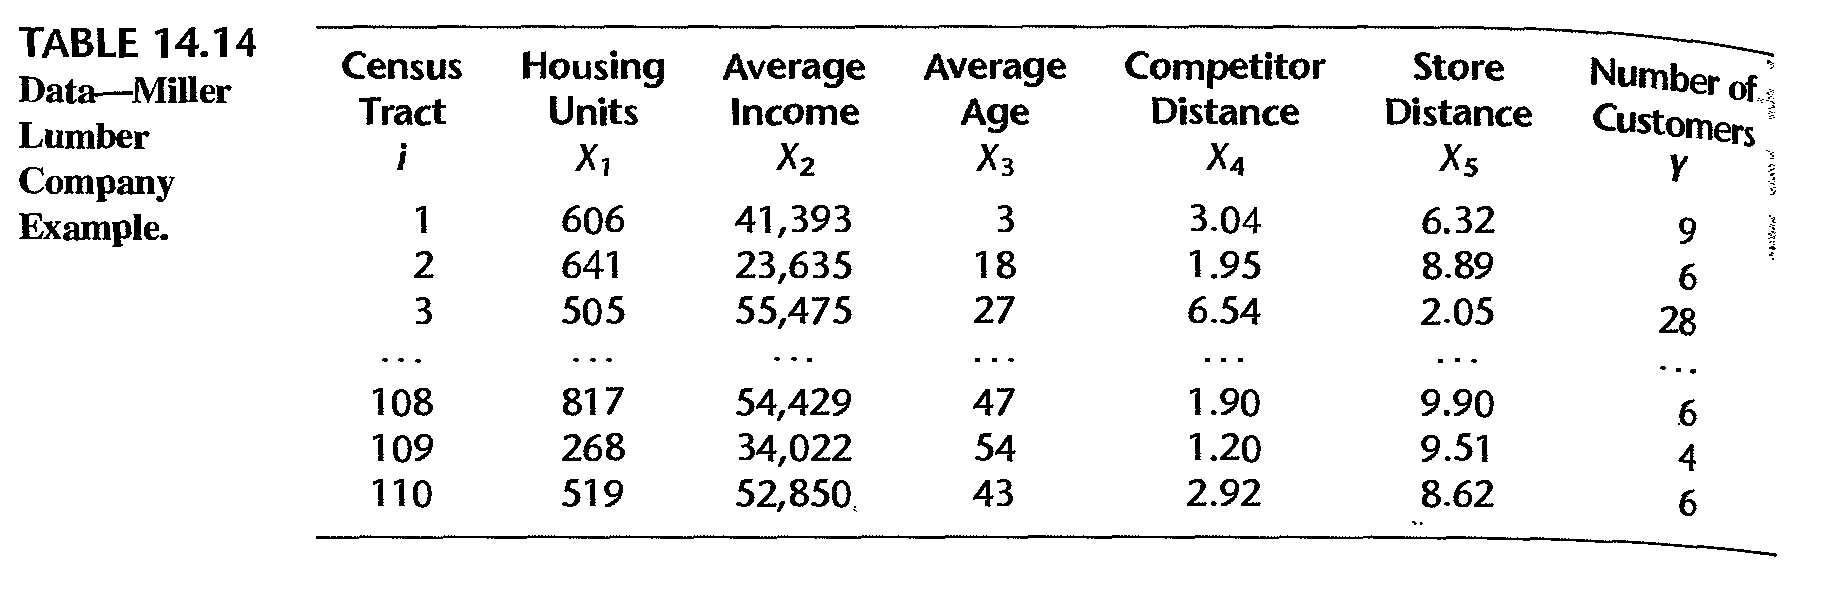
\includegraphics[width=0.85\linewidth]{tab14.14} \end{center}

\subsection{Example: fitted model}\label{example-fitted-model}

\begin{center}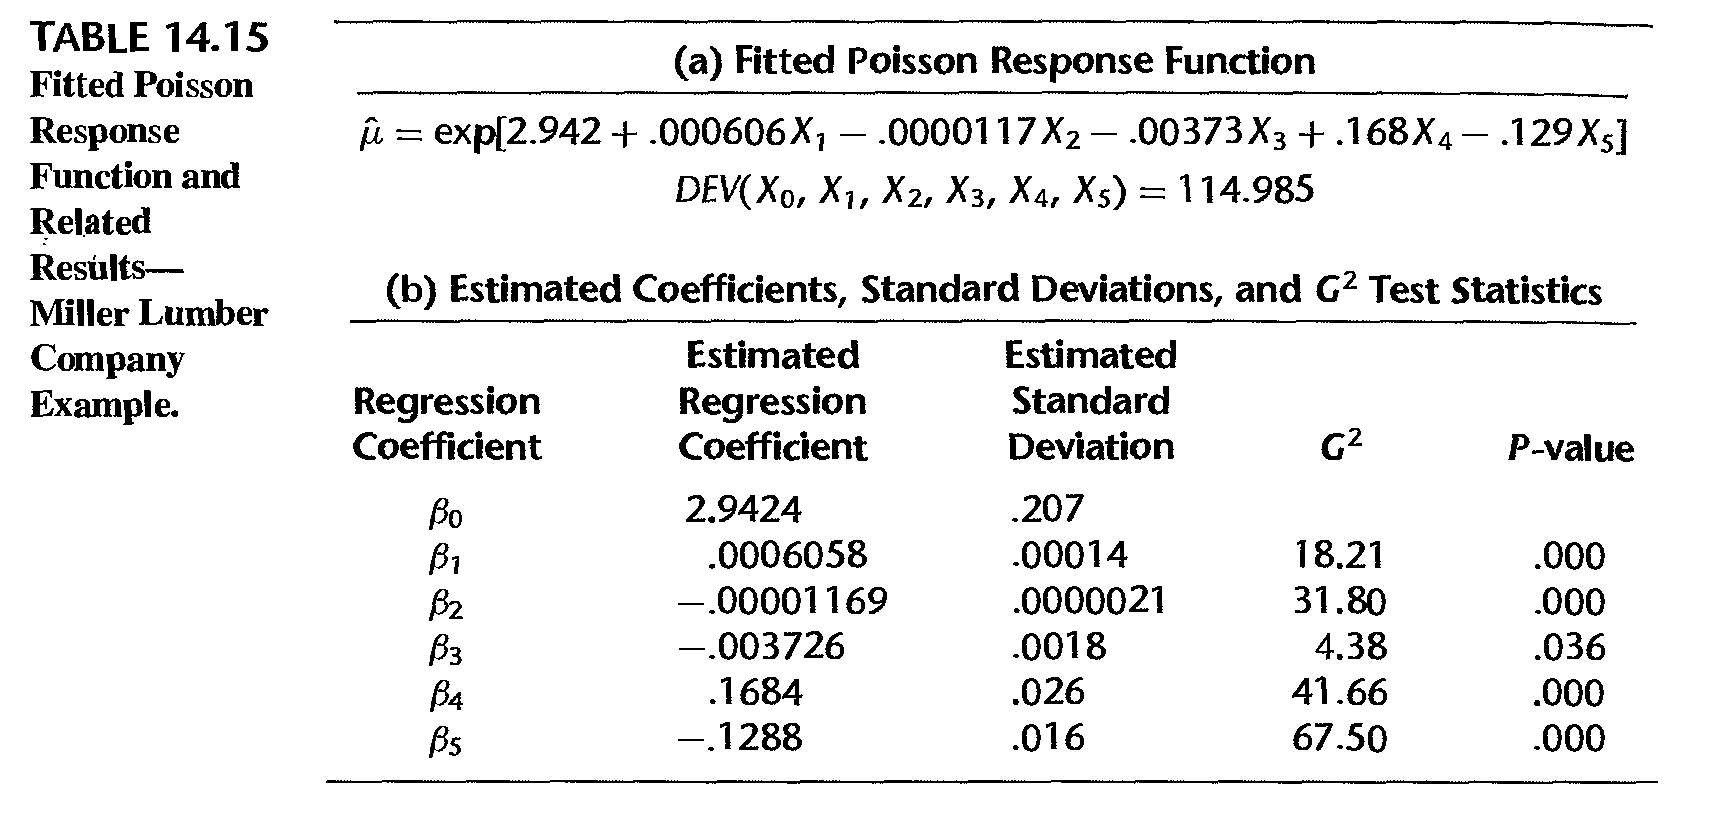
\includegraphics[width=0.85\linewidth]{tab14.15} \end{center}

\begin{itemize}
\tightlist
\item
  \(G^2 = - 2 \ln [L(R)/L(R)] \sim\) chi-square distribution
\end{itemize}

\subsection{Example: diagnosis}\label{example-diagnosis}

\begin{center}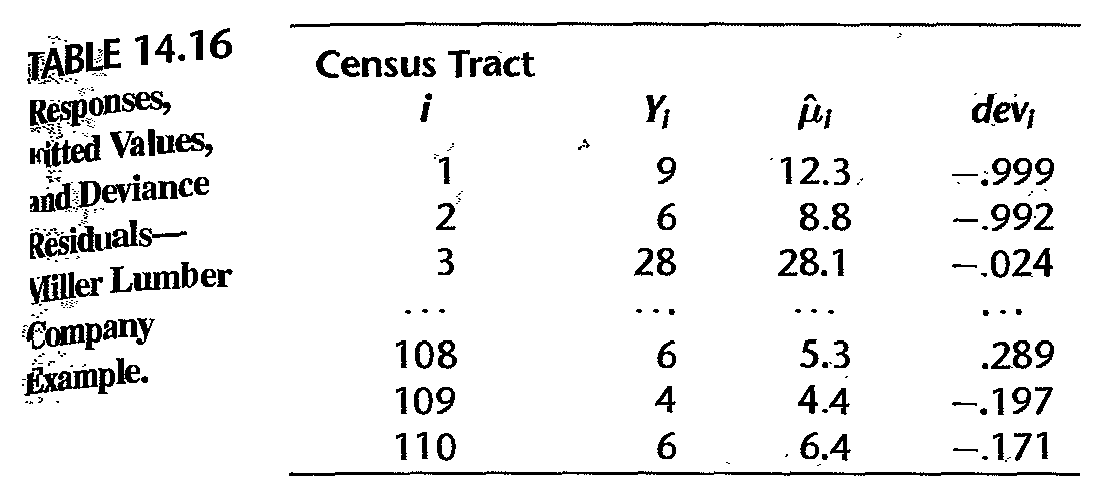
\includegraphics[width=0.85\linewidth]{fig14_16} \end{center}

\begin{itemize}
\tightlist
\item
  deviance residual vs fitted value; table shows no serious issue
\end{itemize}

\subsection{Example: diagnosis}\label{example-diagnosis-1}

\begin{center}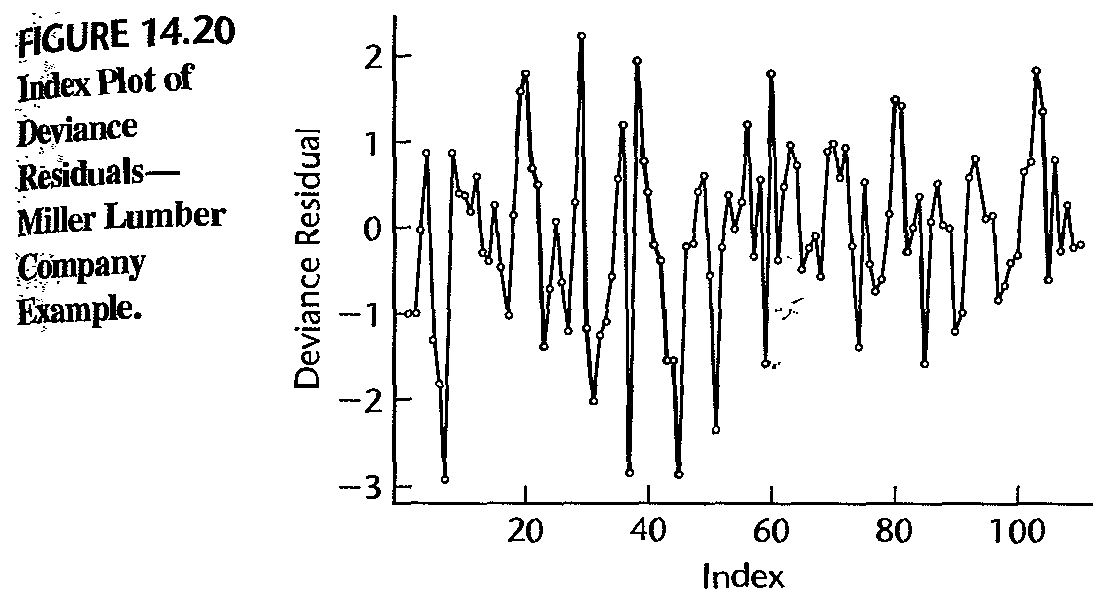
\includegraphics[width=0.85\linewidth]{fig14_20} \end{center}

\begin{itemize}
\tightlist
\item
  a few large negative deviance residuals associated tracts with zero
  customers; hard to fit these values
\end{itemize}

\subsection{License and session
Information}\label{license-and-session-information}

\href{http://math.wsu.edu/faculty/xchen/stat412/LICENSE.html}{License}

\begin{Shaded}
\begin{Highlighting}[]
\NormalTok{>}\StringTok{ }\KeywordTok{sessionInfo}\NormalTok{()}
\NormalTok{R version }\FloatTok{3.5.0} \NormalTok{(}\DecValTok{2018-04-23}\NormalTok{)}
\NormalTok{Platform:}\StringTok{ }\NormalTok{x86_64-w64-mingw32/}\KeywordTok{x64} \NormalTok{(}\DecValTok{64}\NormalTok{-bit)}
\NormalTok{Running under:}\StringTok{ }\NormalTok{Windows }\DecValTok{10} \KeywordTok{x64} \NormalTok{(build }\DecValTok{19044}\NormalTok{)}

\NormalTok{Matrix products:}\StringTok{ }\NormalTok{default}

\NormalTok{locale:}
\NormalTok{[}\DecValTok{1}\NormalTok{] LC_COLLATE=English_United States}\FloatTok{.1252} 
\NormalTok{[}\DecValTok{2}\NormalTok{] LC_CTYPE=English_United States}\FloatTok{.1252}   
\NormalTok{[}\DecValTok{3}\NormalTok{] LC_MONETARY=English_United States}\FloatTok{.1252}
\NormalTok{[}\DecValTok{4}\NormalTok{] LC_NUMERIC=C                          }
\NormalTok{[}\DecValTok{5}\NormalTok{] LC_TIME=English_United States}\FloatTok{.1252}    

\NormalTok{attached base packages:}
\NormalTok{[}\DecValTok{1}\NormalTok{] stats     graphics  grDevices utils     datasets  methods  }
\NormalTok{[}\DecValTok{7}\NormalTok{] base     }

\NormalTok{other attached packages:}
\NormalTok{[}\DecValTok{1}\NormalTok{] knitr_1}\FloatTok{.21}

\NormalTok{loaded via a }\KeywordTok{namespace} \NormalTok{(and not attached):}
\StringTok{ }\NormalTok{[}\DecValTok{1}\NormalTok{] compiler_3}\FloatTok{.5.0}  \NormalTok{magrittr_1}\FloatTok{.5}    \NormalTok{tools_3}\FloatTok{.5.0}    
 \NormalTok{[}\DecValTok{4}\NormalTok{] htmltools_0}\FloatTok{.3.6} \NormalTok{yaml_2}\FloatTok{.2.0}      \NormalTok{Rcpp_1}\FloatTok{.0.12}    
 \NormalTok{[}\DecValTok{7}\NormalTok{] stringi_1}\FloatTok{.2.4}   \NormalTok{rmarkdown_1}\FloatTok{.11}  \NormalTok{stringr_1}\FloatTok{.3.1}  
\NormalTok{[}\DecValTok{10}\NormalTok{] xfun_0}\FloatTok{.4}        \NormalTok{digest_0}\FloatTok{.6.18}   \NormalTok{evaluate_0}\FloatTok{.13}  
\end{Highlighting}
\end{Shaded}


\end{document}
